\chapter{Combinatorics}

Probability theory is about sets. In the first lesson you encountered
the set of possible outcomes of flipping two coins which contains four
elements. If we use $H$ to denote ``Heads'' and $T$ to denote
``Tails'' then the set of possible outcomes, also known as the {\em
  outcome space} contains four elements: $\{(H,H),(H,T),(T,H),(T,T)\}$. We say
that the outcome space is the set of four {\em tuples}. As the
concepts of ``set'' and ``tuple'' will be used many times throughout
the course, we take some pains to define these concepts and the
associated notation, in a somewhat formal mathematical way.

Think of this as learning the syntax and semantics of a new
programming language. There is nothing very deep here, it is just a
framework through which deeper ideas can be expressed precisely and
succinctly.

\iffalse
\begin{figure}[t]
  \centering
  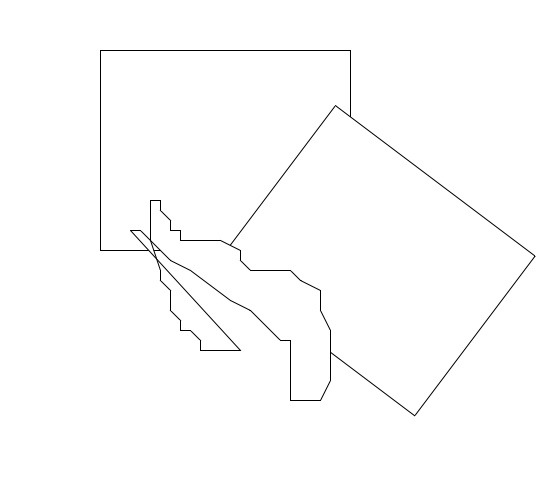
\includegraphics[width=0.45\textwidth]{figs/testImage}
  \caption{test figure}
\end{figure}
\fi
  
\section{Sets}
{\it Sets} are collections of {\it elements}. We will mostly consider sets of
numbers, but elements can be most anything.

A {\it set} can be specified by listing its elements within braces, as in
\begin{align*}
A=\{1,2,3,4,5,6\} &\ (\mbox{the possible outcomes of the roll of a die}) \\
B=\{1,2,\ldots\}  &\ (\mbox{the positive integers, commonly denoted
  $\mathbb{Z}^+$}) \\
C=\{H,T\} & (\mbox{the possible outcomes of the flip of a coin}) 
\end{align*}
We say that $5$ is an element of $A$ and denote it by $5 \in A$. Sets
are {\em unordered} collections, in other words $\{1,2,3,4,5,6\} =
\{5,2,1,3,4,6\}$. The number of times an element can appear in a set
is either 0 or 1, an element cannot appear multiple times in the set
(for that there is a different construct called {\em bags}).

Instead of listing the elements of a set, one can define a set by
specifying the precise conditions for an element to be in the set. For
example:
\begin{align*}
\mathbb{Z}^+ &= \{x: \mbox{$x$ is a positive integer}\} \\
\mathbb{R}   &= \{x: \mbox{$x$ is a real number}\} .
\end{align*}
When set $S$ is contained in set $T$ (that is, $x \in S \Rightarrow x
\in T$), we write $S \subseteq T$. For instance, $\mathbb{Z}^+
\subseteq \mathbb{R}$. The {\em empty set} contains no elements and is
denoted by $\{\}$ or $\emptyset$.

Suppose $A,B$ are two sets. The {\em intersection} of the two sets,
denoted $A\cap B$ contains the elements that are in {\em both}
sets. Thus
\begin{align*}
\{1,2,3,4,5,6\} \cap \{2,4,6,8,10\} = \{2,4,6\}
\end{align*}
The {\em union} of two sets contains those elements that are {\em
  either} $A$ or $B$ (or both), thus
\begin{align*}
\{1,2,3,4,5,6\} \cup \{2,4,6,8,10\} = \{1,2,3,4,5,6,8,10\}
\end{align*}

\subsection{Spaces and complements}
In probability we call the set of all possible outcomes (for a
particular experiment) as {\em the outcome space} and denote it by
$\Omega$. Subsets of $\Omega$ are called {\em events}. The {\em
  complement} of an event $A$ is the set of outcomes that are in
$\Omega$ but not in $A$. The complement of the set $A$ is denoted
$A^c$. For example, suppose $\Omega=\{1-10\}$ then 
\subsection{Tuples, and products of sets}

Suppose we toss a coin three times. We can represent the outcome by a 3-tuple like
$(H,H,T)$ (where $H$ means heads and $T$ means tails). The set of all
such tuples is
$$ 
\{(H,H,H), (H,H,T), (H,T,H), (H,T,T), (T,H,H), (T,H,T), (T,T,H), (T,T,T)\}.
$$
It can also be written as $\{H,T\} \times \{H,T\} \times \{H,T\}$, or even more 
simply, $\{H,T\}^3$.

More generally, if $S_1, S_2, \ldots, S_k$ are sets, then 
$S_1 \times S_2 \times \cdots \times S_k$ is the set of all $k$-tuples in which
the first entry is from $S_1$, the second entry is from $S_2$, and so on. For
instance,
\begin{align*}
\mathbb{R}^2 &= \{\mbox{all points in the plane}\} \\
\mathbb{R}^d &= \{\mbox{all points in $d$-dimensional space}\} .
\end{align*}

Note that, unlike sets, {\em order} is significant in tuples. Also
note that the same element can appear multiple times in a tuple, but
not in a set.

We are often also interested in sets of tuples that cannot be expressed as 
products of individual sets. For instance, the points in the unit circle in
$\mathbb{R}^2$ are
$$ \{(x,y): x^2 + y^2 \leq 1 \},$$
a subset of $\R^2$ that cannot be written as a product $S_1 \times S_2$.

\subsection{The size of a set}

The {\em size} of a set $A$ is the number of elements in it and is denoted
by $|A|$. Thus $|\{H,T\}|=2$, $|\emptyset|=0$ and $|\mathbb{Z}^+|=\infty$.

When $S$ is of the form 
$S_1 \times \cdots \times S_k$, then
$|S| = |S_1| \cdot |S_2| \cdots |S_k|$.

To see an example of this notation, suppose there is a group of $n$
concert-goers, each of whom is selecting a band T-shirt. The available
colors are red, yellow, and black. How many possible outcomes are
there? Well, let $C = \{\mbox{red}, \mbox{yellow}, \mbox{black}\}$ be
the set of possible colors, and represent each outcome as an $n$-tuple
in which the $i$th entry is the color of the $i$th person's T-shirt.
Then the possible outcomes are $C^n$, a set of size $|C|^n = 3^n$.

\section{Permutations and combinations}

Armed with the concepts of sets, tuples and set size we can now tackle
some more interesting combinatorial questions.

\subsection{Sampling with and without replacement when the order matters}

Suppose there are four children---Alice, Bill, Christie, and Doug---at an animal
shelter, checking out the current pool of $n$ dogs. Each child writes down the 
name of the dog he or she likes most. How many possible outcomes are there?

We can represent each outcome as a 4-tuple (Alice's choice, Bill's choice,
Christie's choice, Doug's choice) in which each entry is the name of a dog. 
So the number of outcomes is $n^4$.

Now suppose that these same children are actually picking out dogs. First Alice 
chooses a dog to adopt, then Bill chooses a dog to adopt, and so on. How many 
outcomes are there now?

In this situation, Alice has $n$ choices, but Bill has only $n-1$ choices,
Christie has $n-2$ choices, and Doug has $n-3$ choices. So there are
$n(n-1)(n-2)(n-3)$ possible outcomes.\\

The first situation is called {\it sampling with replacement}: the
outcomes are tuples in which the same element (dog) can occur more
than once. The number of such $k$-tuples, chosen from $n$ elements, is
$n^k$. In the example, $k=4$. The second situation is {\it sampling
  without replacement}: the outcomes are tuples in which no element
can be repeated. The number of such $k$-tuples, chosen from $n$
elements, is $n(n-1)(n-2) \cdots (n-k+1)$. \\

Here's a related question: how many ways are there to order (shuffle)
a deck of 52 cards?  (Each such ordering is called a {\it permutation}
of the cards.) Well, the result is a 52-tuple, drawn from a set of
size 52, in which no card is repeated. Therefore, the number of
permutations is $52 \cdot 51 \cdot 50 \cdots 1$, which is called $52$
{\em factorial} and denoted as $52!$. More generally, the number of
permutations of $n$ elements is $n$ factorial or $n!$.

Coming back to sampling $k$ out of $n$ elements without replacement,
we can write it succinctly as 
\[
n(n-1)(n-2) \cdots (n-k+1) = \frac{n!}{(n-k)!}
\]

\subsection{When the order doesn't matter}

Snow White is off to pick strawberries and asks three of the dwarfs (chosen 
from the seven: Dopey, Grumpy, Doc, Happy, Bashful, Sneezy, Sleepy) to join 
her. How many possible groups are there?

In this case, it is misleading to represent an outcome as a 3-tuple, because, 
for instance, $\mbox{(Dopey, Sleepy, Doc)}$ is a different 3-tuple from
$\mbox{(Sleepy, Dopey, Doc)}$ but they represent the same group. So if we count
tuples, we would be {\it over-counting}. Instead, we ought to represent an 
outcome as a set, $ \{\mbox{Dopey, Doc, Sleepy}\}$.

So the question becomes: how many different subsets of three dwarfs are there?
In general, a set of size $n$ has 
$${n \choose k} \ = \ \frac{n!}{k! (n-k)!} $$ 
subsets of size $k$. So in our example, the answer is ${7 \choose 3} = 35$.
\\

Let's step back and derive the main result: how many subsets of size $k$ does a
set of $n$ elements have? We can choose the subset in the following manner: first
pick one element from the set, then a second (different) element, then a third 
(different) element, and so on until we have $k$ distinct elements. This yields 
a $k$-tuple (first choice, second choice, etc), and as we saw above (sampling
without replacement when the order matters) the number of possible such tuples 
is $n(n-1) \cdots (n-k+1)$. However, we have over-counted because each subset of 
size $k$ appears multiple times amongst these $k$-tuples. To be precise, each 
subset corresponds to exactly $k!$ tuples, depending on the order in which the 
$k$ elements of the subset are chosen. Thus the number of subsets of size $k$ is
$$ \frac{n(n-1)\cdots (n-k+1)}{k!} \ = \ \frac{n!}{k!(n-k)!} .$$
\\

A second example: how many strings in $\{0,1\}^{10}$ contain exactly
{\it four} 1s?  Well, we need to choose four positions of the ten
possibilities in which to place the 1s; that is, we choose a subset of
size four from $\{1,2,\ldots,10\}$.  The number of ways to do this is
${10 \choose 4} = 210$.
\\

Let's finish with a more challenging example. You walk into a candy
store and notice that there are five types of candy. Your mother
allows you to pick exactly three pieces of candy, of whichever type(s)
you want. How many ways are there to do this?

You can represent the outcome by 5-tuple $(n_1, n_2, \ldots, n_5)$ in
which $n_i$ is the number of pieces of the $i$th type of candy. How
many such tuples are there, subject to $n_1 + n_2 + \cdots + n_5 = 3$?
To answer the question, we'll represent each tuple in a different
format, as a sequence of length 7 containing three stars and four
bars. For instance, the sequence $|\,**\,|\,|\,|\,*$ denotes
$(0,2,0,0,1)$ (two candies of type 2 and one candy of type 5): the
number of candies of type $i$ is the number of stars between the
$(i-1)$st and $i$th bars.
 
So we have rephrased the question thus: how many sequences are there
with four bars and three stars? Well, this is a sequence of size 7,
and we must pick three of the seven positions at which to place
stars. The number of such choices is ${7 \choose 3} = 35$.

